\documentclass[9pt,twocolumn]{article}

\usepackage[a4paper,margin=0.55in,columnsep=0.20in]{geometry}
\usepackage{amsmath,amssymb}
\usepackage{booktabs}
\usepackage{graphicx}
\usepackage{xcolor}
\usepackage{hyperref}
\usepackage{enumitem}
\usepackage[font=small,labelfont=bf]{caption}
\captionsetup{skip=2pt}

\hypersetup{colorlinks=true,urlcolor=blue,linkcolor=blue,citecolor=blue}
\setlist{nosep,leftmargin=*}
\setlength{\parindent}{0.8em}
\setlength{\parskip}{0pt}

\title{\vspace{-1.2em}\textbf{DockRush: Deadline-Aware Warehouse Fulfilment with Reinforcement Learning}}
\author{\textbf{Team:} Mohi1038 (B23CS1038) and Nidhish Bhatt (B23CS1009) \quad
\href{https://github.com/Mohi1038/rl-warehouse-fulfillment}{GitHub repository}}
\date{}

\begin{document}
\maketitle
\vspace{-1.5em}

\begin{abstract}
DockRush formulates warehouse order fulfilment as a practical reinforcement-learning
problem. A robot receives stochastic orders, picks items, delivers them to docks before
truck departures, and manages capacity and battery constraints. We model this as an
event-driven semi-Markov decision process (SMDP), where actions have different durations.
The main agent is a masked PPO policy with a permutation-invariant attention encoder and
pointer-style order selection. On 100 held-out seeds, PPO-Attention obtains
$153.0\pm3.9$ task return, 67.3\% revenue captured, and 78.3\% express-order on-time
delivery, outperforming DQN and evaluation baselines.
\end{abstract}

\section{Problem and Unique Ideation}
The practical problem is deciding which warehouse task a robot should perform next when
orders arrive over time and trucks leave at uncertain deadlines. The project is intentionally
RL-only: PPO, DQN, and tabular Q-learning are the learning methods; FIFO, EDF, Greedy, and
Random are used only as evaluation reference policies, not as the proposed solution.

The distinctive design is the combination of five elements in one RL environment:
\begin{enumerate}
\item stochastic non-homogeneous order arrivals with midday demand peaks and rush shocks;
\item hidden truck-departure jitter, express/standard/bulk priorities, and order deferral;
\item variable-duration macro-actions, making the problem an SMDP rather than a fixed-step toy grid;
\item a hard action mask for invalid picks, unsafe battery moves, and empty deliveries; and
\item a permutation-invariant attention policy that can run with larger order queues than seen
      during training, plus a shared asynchronous multi-robot extension.
\end{enumerate}
This is a system-level ideation contribution rather than a claim of a new PPO theorem:
the originality is in the realistic RL formulation, the deadline-sensitive reward design,
and the stress tests that measure generalisation, ablations, and fleet scaling.

\section{RL Formulation}
\subsection{State space $\mathcal{S}$}
At each decision event, the observation is a dictionary:
\[
s_t=(g_t,O_t,M_t[,R_t]).
\]
For the nominal single-robot setting, $g_t\in\mathbb{R}^{16}$ contains normalized time
(including sine/cosine phase), battery, load, position, carried orders per dock, dock
countdowns, backlog, recent arrival rate, and capacity. The order matrix is
$O_t\in\mathbb{R}^{16\times14}$: each of 16 slots contains presence, value, tier,
destination dock, deadline slack after an estimated completion time, remaining items,
carried/loaded items, distance, capacity feasibility, and age features. $M_t$ is a
binary action mask. In multi-robot experiments, $R_t\in\mathbb{R}^{3\times12}$ contains
robot identity, position, target, load, battery, and busy-time tokens. All continuous
features are normalized and padded slots are zero.

\subsection{Action space $\mathcal{A}$}
The action space is discrete:
\[
\begin{aligned}
\mathcal{A}={}&\{\operatorname{PICK}(i):i=1,\ldots,N_{\max}\}\\
&\cup\{\operatorname{DELIVER}(d):d=1,\ldots,D\}\\
&\cup\{\operatorname{CHARGE},\operatorname{WAIT}\}.
\end{aligned}
\]
With $N_{\max}=16$ and $D=3$, there are 21 actions. A selected action is executed until
the corresponding event completes, so its duration $\tau_t$ varies with travel distance,
item count, picking, loading, charging, or waiting. The mask removes impossible or unsafe
choices; masked logits are excluded before sampling.

\subsection{Reward function}
For one option, the environment logs fulfilled, lost, and deferred orders. The reward is
\[
r_t=F_t-\lambda_m L_t-\frac{\lambda_d}{2}D_t
 -\lambda_c\tau_t K-\lambda_b I_t+\alpha\bigl(\Phi(s_{t+1})-\Phi(s_t)\bigr),
\]
where $F_t$ is fulfilled order value, $L_t$ is missed-order loss, $D_t$ is deferred
value, $K$ is the number of robots, and $I_t$ indicates a stranded battery. The default
coefficients are $\lambda_m=1$, $\lambda_d=0.3$, $\lambda_c=0.01$, $\lambda_b=50$, and
$\alpha=0.3$. The potential $\Phi$ rewards progress toward loading valuable orders and
carrying orders that can still reach their dock before departure. This encourages useful
progress without replacing the task return used for final comparison.

\subsection{SMDP transition and objective}
The simulator uses a 720-tick shift on a grid warehouse. Orders follow a thinning-based
non-homogeneous Poisson process; trucks depart every 120--180 ticks with Gaussian timing
jitter. The robot has capacity 6 and battery capacity 400. The SMDP-correct choice is
duration-aware discounting in GAE:
\[
\gamma_t=\gamma^{\tau_t},\qquad
\delta_t=r_t+\gamma_t V(s_{t+1})-V(s_t).
\]
With $\gamma=0.995$ per tick this spans only about 20 decisions, so the final PPO agent
uses a per-decision discount $\gamma_t=\gamma$, which trained better
(Section~\ref{sec:results}).

\section{Algorithms and Evaluation}
The primary learner is PPO with clipped policy updates, value loss, entropy regularization,
gradient clipping, vectorized environments, masked actions, and the attention encoder.
The encoder treats order slots as a set and uses a learned \texttt{[CLS]} token to produce
the policy context; a pointer head scores each order slot. DQN uses a dueling double-Q
network, prioritized replay, n-step returns, the same observation/action mask, and the
duration-aware discount. Tabular Q-learning is used only in a tiny exact-check
environment.

Training uses five independent seeds for the main agents and three for ablations. Final
results use 100 held-out evaluation seeds disjoint from checkpoint selection. We compare
nominal performance, unseen layouts, arrival-rate/capacity grids, larger queues, six
ablations, attention behavior, a tiny near-optimality check, and one-to-three robots.

\begin{figure}[t]
\centering
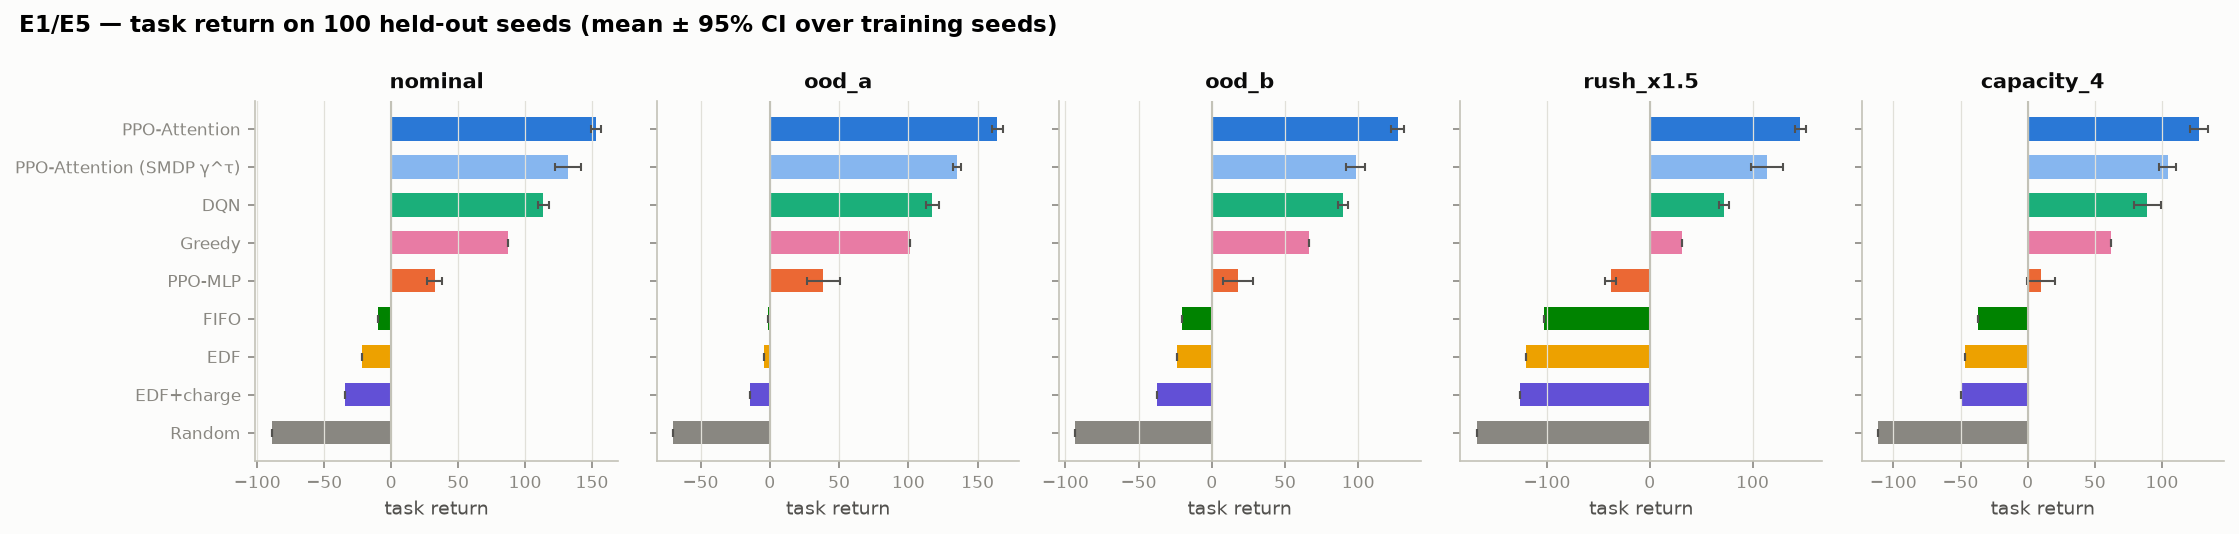
\includegraphics[width=0.96\linewidth,height=0.72in,keepaspectratio]{figures/e1_e5_benchmark.png}\\[2pt]
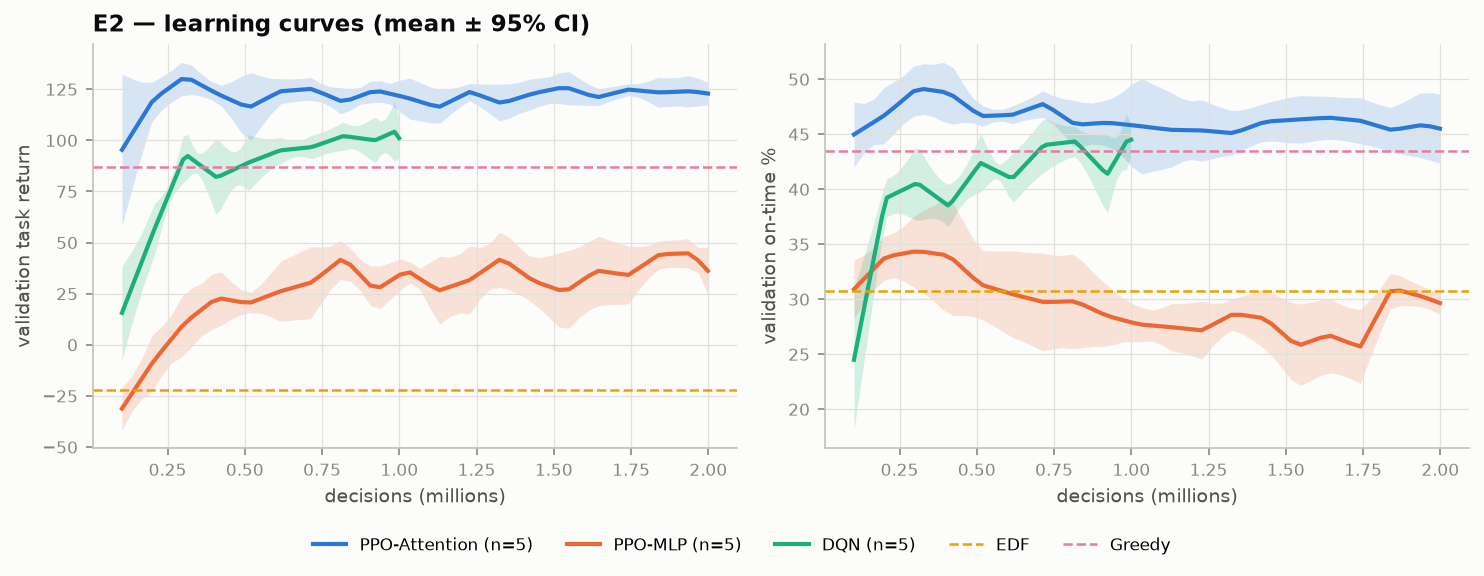
\includegraphics[width=0.96\linewidth,height=0.72in,keepaspectratio]{figures/e2_learning_curves.png}\\[2pt]
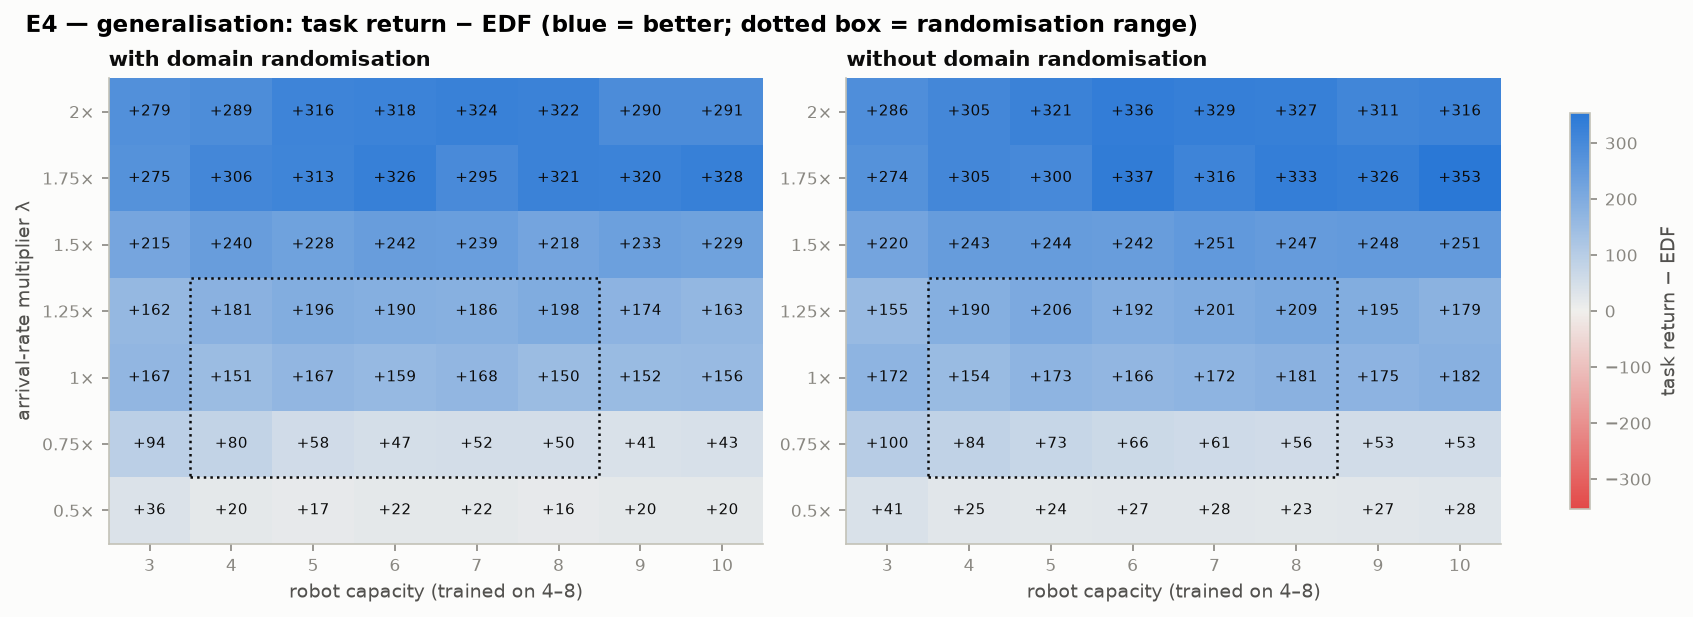
\includegraphics[width=0.96\linewidth,height=0.72in,keepaspectratio]{figures/e4_generalisation.png}
\caption{Benchmark, learning curves, and out-of-distribution generalisation.}
\label{fig:results}
\end{figure}

\begin{figure}[t]
\centering
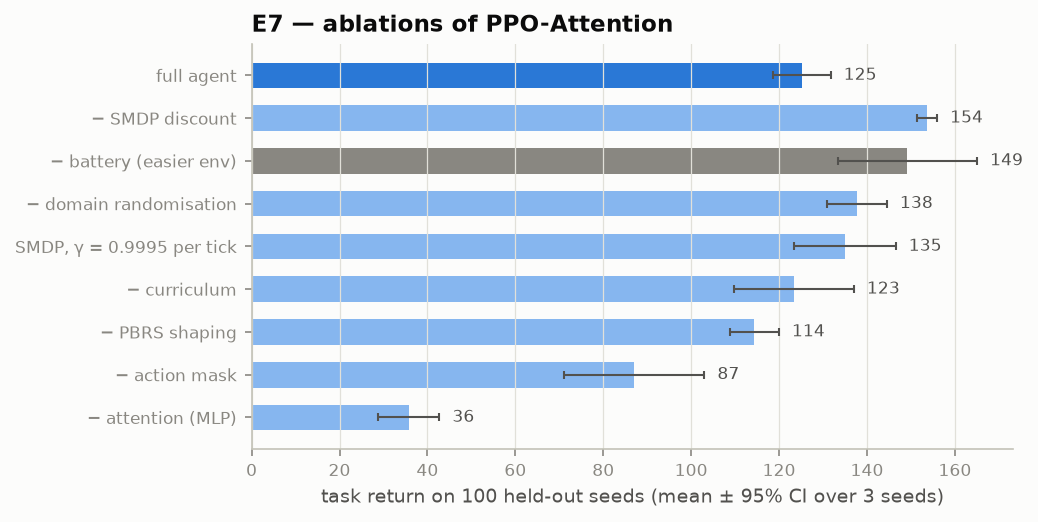
\includegraphics[width=0.96\linewidth,height=0.72in,keepaspectratio]{figures/e7_ablations.png}\\[2pt]
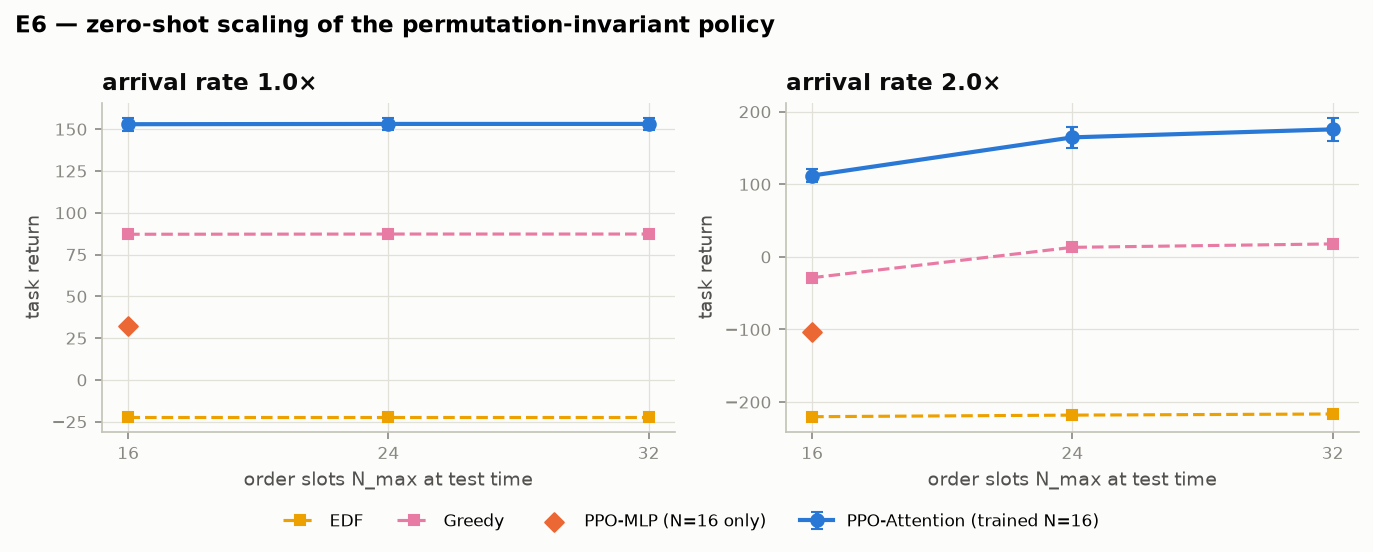
\includegraphics[width=0.96\linewidth,height=0.72in,keepaspectratio]{figures/e6_scaling.png}\\[2pt]
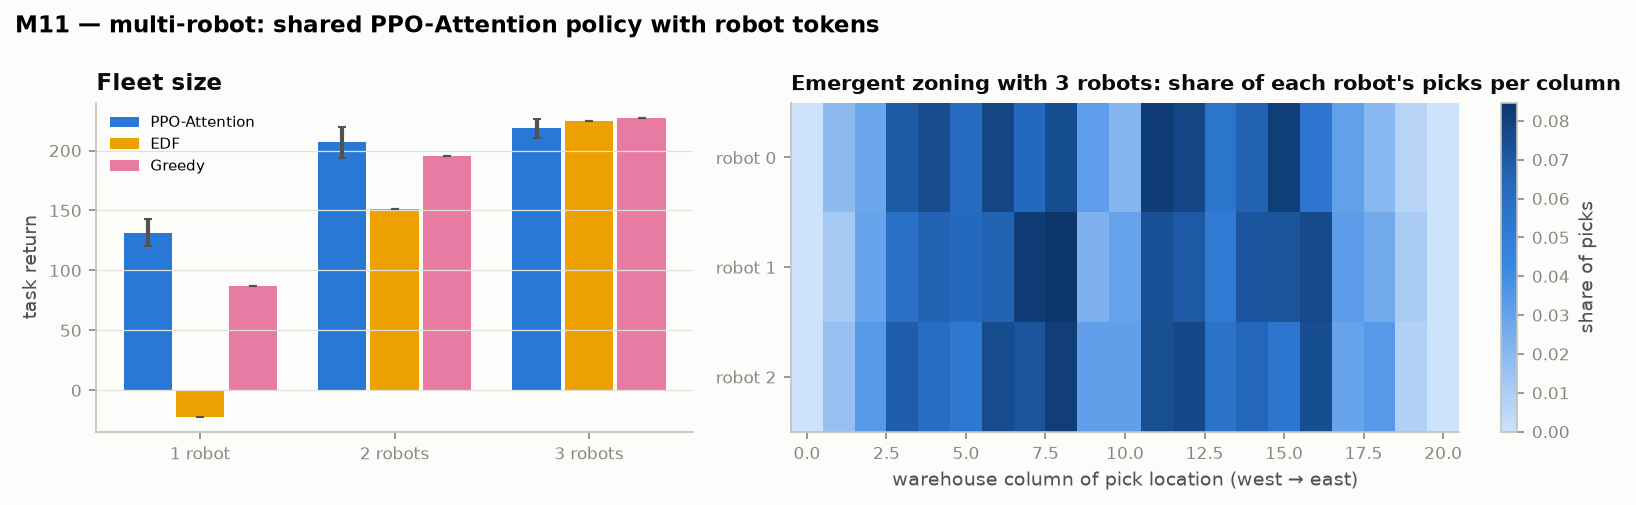
\includegraphics[width=0.96\linewidth,height=0.72in,keepaspectratio]{figures/m11_multi_robot.png}
\caption{Ablations, zero-shot scaling, and multi-robot results.}
\label{fig:scaling}
\end{figure}

\section{Results and Discussion}
\label{sec:results}
PPO-Attention is the strongest nominal policy and retains its advantage on unseen layouts,
arrival-rate changes, and capacity changes. Its express on-time rate is 78.3\%, compared
with 54.6\% for Greedy. The attention policy also transfers from 16 training slots to
24 and 32 test-time slots. The ablation study (on the original agent) shows that removing
attention reduces task return by about 89 points and removing the action mask by about 38
points, supporting the importance of set-based order selection and feasibility-aware decisions.

A per-decision discount raised task return from $132.0\pm9.5$ to $153.0\pm3.9$ and revenue
from 60.2\% to 67.3\%; a $5\times$ larger network did not help. Look-ahead over 32 sampled
futures lifts the best checkpoint from 66.4\% to 71.0\% revenue (${\approx}3$\,s/decision).

The project also tests an applied multi-robot extension with a shared policy and order
claiming, trained with the original discounting. Two robots reach $207.1\pm12.9$ task return versus $131.6\pm10.9$ for one
robot. With three robots, the system becomes less capacity-bound and all policies
approach high on-time fulfilment. These tests measure whether the formulation remains
useful beyond a single robot, rather than relying only on one curated scenario.

\subsection{Interpretation and limitations}
The attention weights provide a useful diagnostic rather than a separate supervision
signal: express orders receive approximately 2.0 times their uniform attention share,
and orders likely to miss their truck are picked less than half as often as those with
ample slack. The gain over Greedy comes from express orders and 21\% less travel per order.

There are important limits to the claim. The warehouse is a simulator, so its demand
model and reward weights are assumptions rather than measurements from a live facility.
The policy is trained on a finite family of layouts and does not solve arbitrary warehouse
maps without retraining or transfer. Finally, the three-robot experiment uses a shared
policy and an order-claiming mechanism; it is evidence of scalability, not a proof of
optimal multi-agent coordination. These limitations motivate future work with logged
warehouse traces, learned demand calibration, communication costs, and safety evaluation
on physical robots.

\subsection{Why reinforcement learning is appropriate}
The best action depends on delayed consequences: picking an order now consumes capacity,
changes the route, affects battery feasibility, and may protect or miss a future truck.
The arrival process is only partially predictable because departure jitter is hidden.
Consequently, a supervised target action is not available for each state, and a static
shortest-path or priority rule cannot optimize the long-term trade-off. PPO learns this
trade-off from repeated interaction using only rewards generated by the environment.
The heuristic policies are therefore useful controls, while the proposed decision-maker
remains an RL policy.

All code, configurations, trained checkpoints, evaluation data, figures, and complete
reproduction commands are provided in the
\href{https://github.com/Mohi1038/rl-warehouse-fulfillment/blob/main/README.md}{GitHub README}.

\section*{References}
\small
\begin{enumerate}\setlength{\itemsep}{0pt}\setlength{\parsep}{0pt}
\item Schulman et al., ``Proximal Policy Optimization Algorithms,'' arXiv:1707.06347, 2017.
\item Sutton and Barto, \emph{Reinforcement Learning: An Introduction}, 2nd ed., 2018.
\item Sutton et al., ``Policy Gradient Methods for Reinforcement Learning with Function Approximation,'' NeurIPS, 2000.
\item Puterman, \emph{Markov Decision Processes}, Wiley, 1994.
\end{enumerate}

\end{document}
